\chapter{Motions of stars}\label{chap:motions}
\begin{flushright}
\textit{``The stars are far brighter, Than gems without measure."}

- J. R. R. Tolkien, The Hobbit
\end{flushright}
\section{The oldest science}\label{sec:oldest}
\begin{figure}[t]
    \centering
    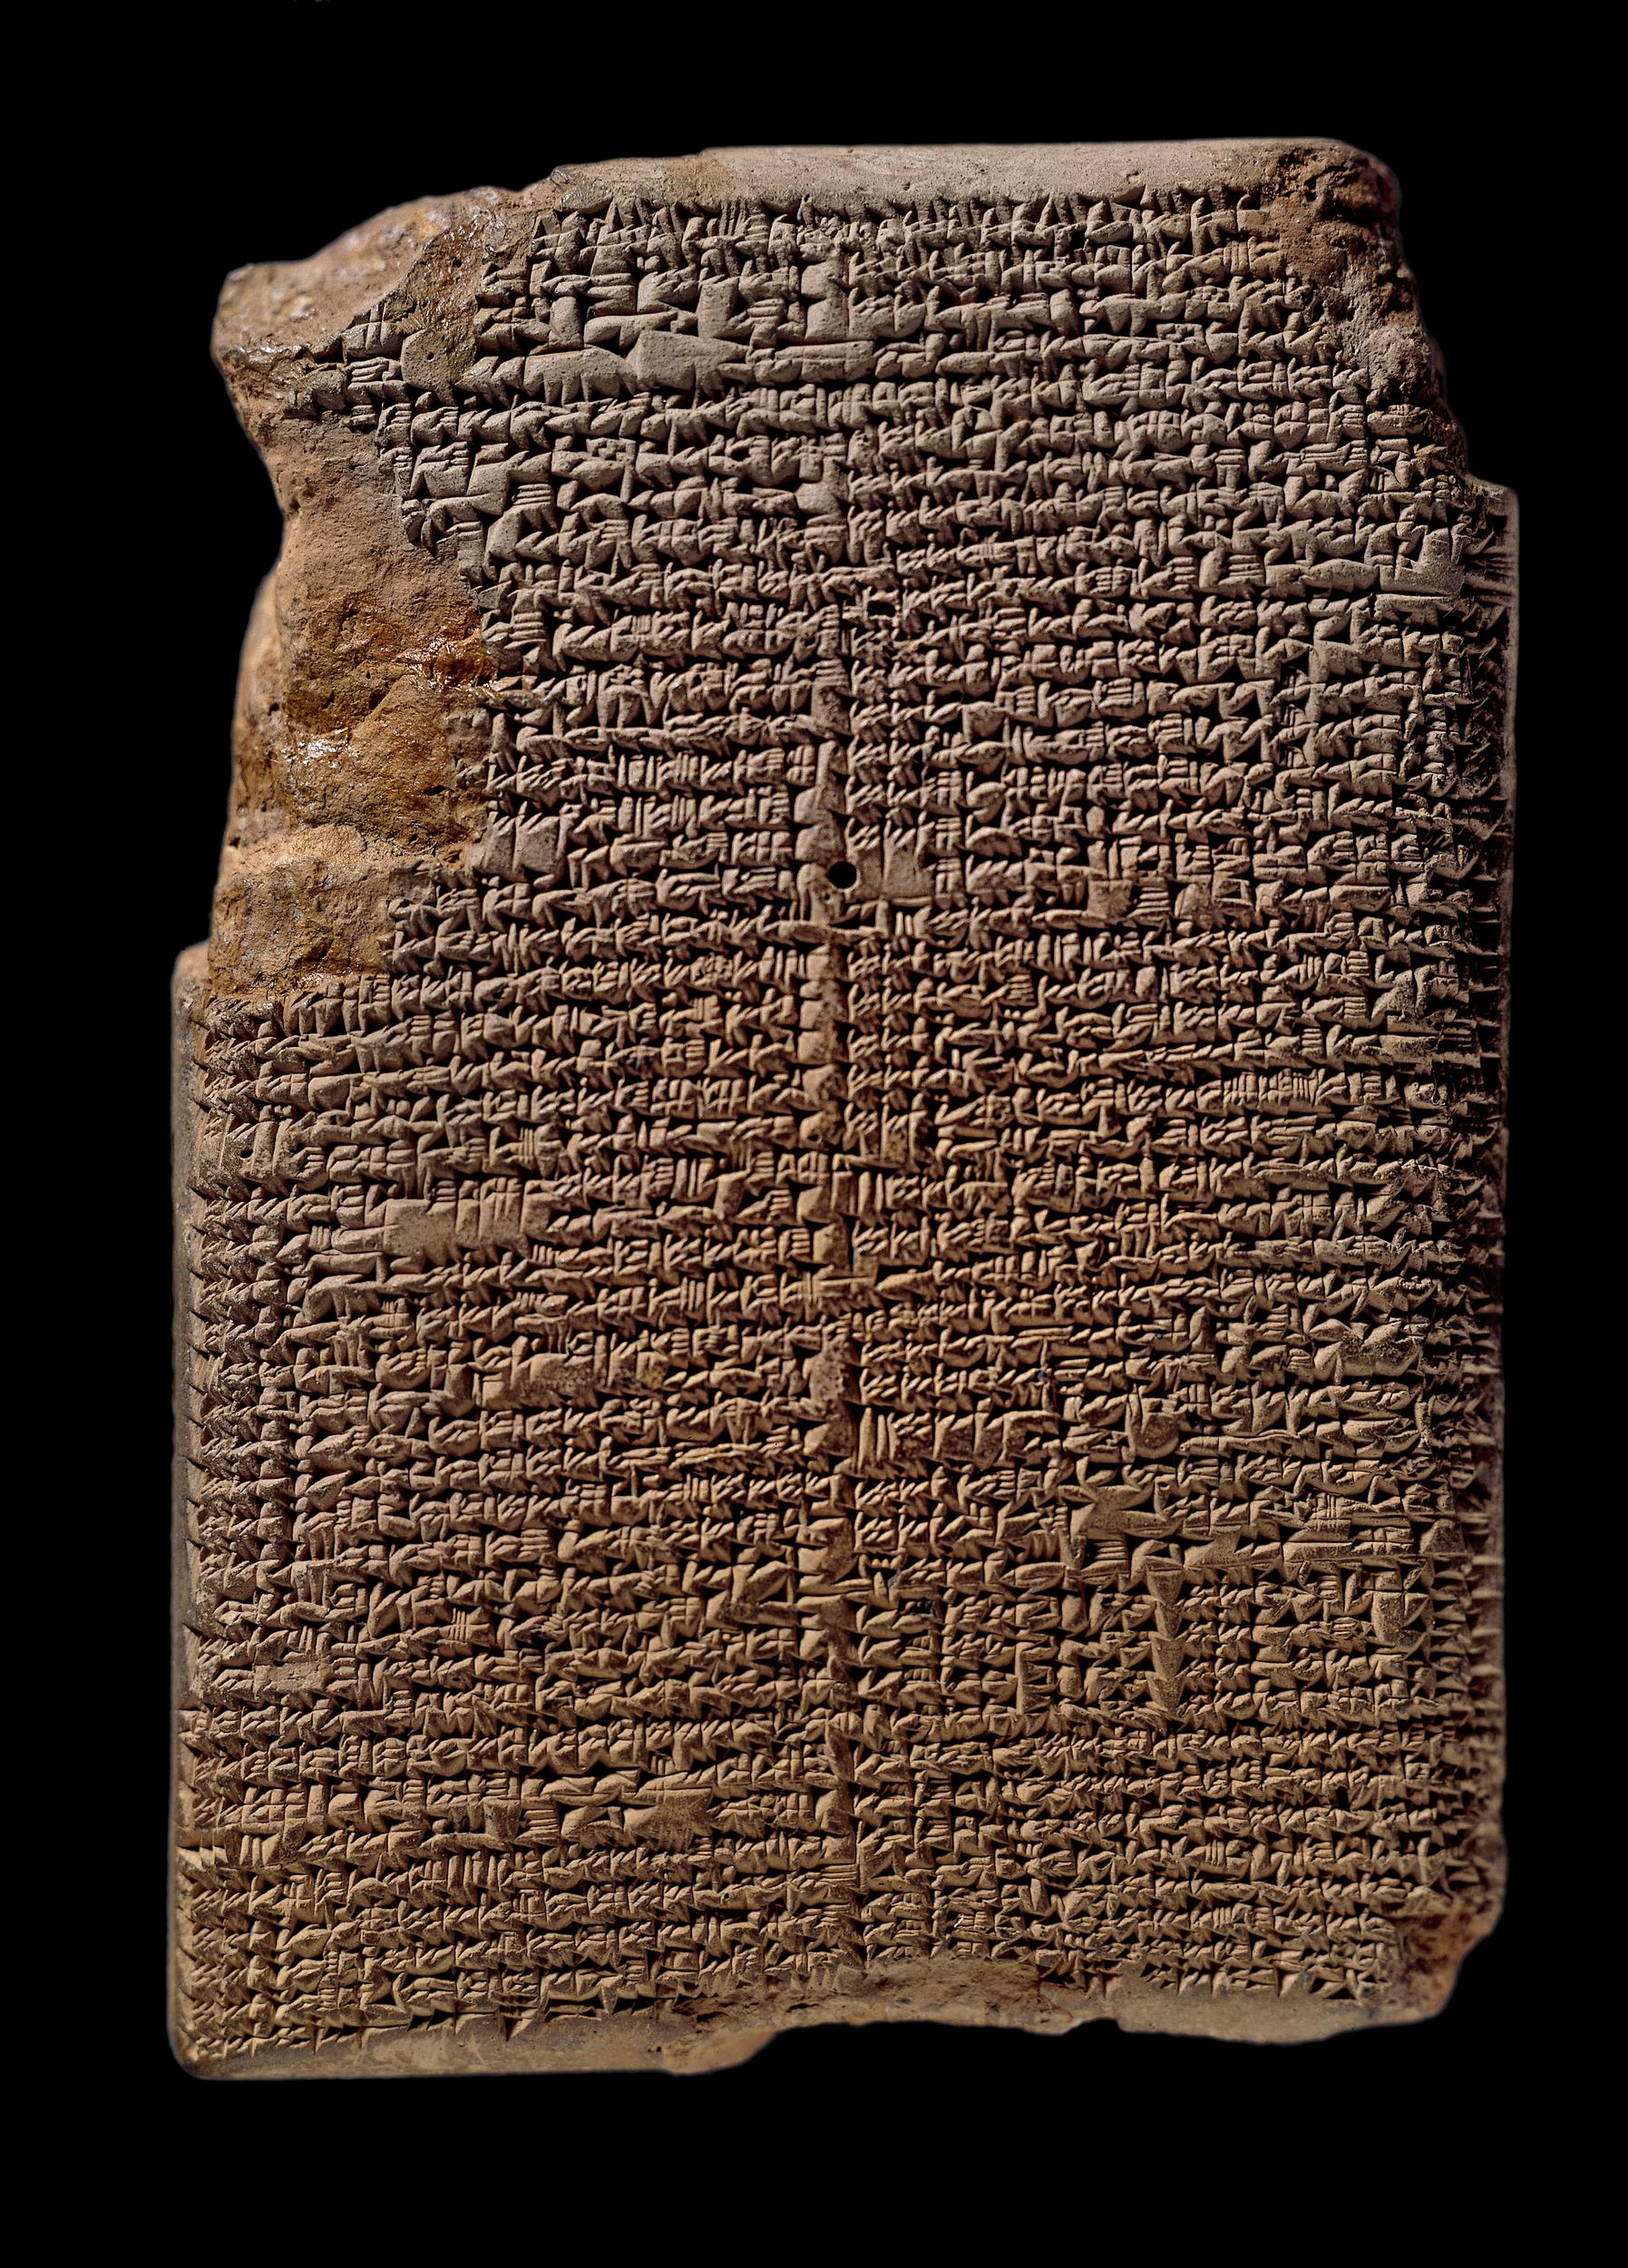
\includegraphics[width=0.4\textwidth]{images/tablet.jpeg}
    \caption{The Mul-Apin clay tablet, tablet 1. The tablet has sections locating constellations in relation to each other and lists stars and constellations according to celestial latitude among other entries. © The Trustees of the British Museum. Shared under a Creative Commons Attribution-NonCommercial-ShareAlike 4.0 International (CC BY-NC-SA 4.0) licence.} % Fig. 3.1
    \label{fig:tablet}
\end{figure}
The fascination of mankind with the celestial sphere has undoubtedly been around for far longer than historical records can demonstrate. Beyond a scientific curiousity, the night sky has had practical purposes that have been used throughout history. Polaris points the way north for travellers of all sorts. The blurring of stars can tell sailors that it is windy at sea. Agriculture heavily relies on the use of calendars based around the Sun and Moon. The relationship between astronomy and humans was arguably more tangible and transparent in the past than it is today, when non-astronomers do not need to think about these matters very often. 

In the last few decades, the study of prehistoric astronomy has boomed into its own field called archaeoastronomy, and revolves around the study of prehistoric sites and their possible astronomical association (see \citealt{magli:20} for a review). These sites have origins dating back several millenia BCE. The earliest historically verified accounts of astronomy comes from Mesopotamia and the ancient kingdoms of Sumer, Assyria, and Babylonia. From this region has been found clay tablets noting down positions and locations for constellations and planets. One significant example of such is the \textit{Mul-Apin} clay tablet, shown in Fig. \ref{fig:tablet}, which dates back to a little over 1000 BCE \citep{dejong:07}. 

Around 200 BCE the first star catalogue was made by \textit{Hipparchus} in ancient Greece\footnote{The history of astrometry is described in much greater detail in \cite{perryman:12} than it is here and we encouraged the interested reader to have a look.}. This catalogue contained positions of stars and is often linked to the birth of \textit{astrometry} as a subject, the study of positions and movements of celestial bodies with precise measurements. As the Roman empire fell and the Dark Ages began, astrometric advances were made to wait. In 1428 a 36-meter sextant was constructed in Uzbekistan by the grandson of the Mongol conqueror Tamarkand, \textit{Ulugh Beg}. This provided a new star catalogue of 994 stellar positions accurate to a degree. The next advancement came from Scandinavia as \textit{Tycho Brahe} (1546-1601) on the Danish island of Hven, using a quadrant of around seven meters at his Uraniborg observatory, measured a thousand stellar positions. His accuracy reached about 20\as. In order to perfect the art of navigation, it was necessary to determine longitude of various places. For this purpose the Royal Greenwich Observatory was founded in 1675 and its first Astronomer Royal was \textit{John Flamsteed} (1646-1719), tasked with determining the motions of the heavens. After his passing was published a catalogue of 2935 stellar positions accurate to 10\as-20\as, the \textit{Historia Coelestis Brittanica} \citep{flamsteed:1725}, the first catalogue using a telescope. This expanded rapidly thereafter and had reached 50 000 stars with 3\as accuracy in \textit{Histoire Céleste Française} by \textit{Jérôme Lalande} (1732 - 1807) \citep{lalande:1801}. 

The next step is not an increasingly large catalogue. Instead, through separate works by \textit{Wilhelm Struve} (1793-1864), \textit{Friedrich Bessel} (1784-1846), and \textit{Thomas Henderson} (1798-1844) the first stellar parallaxes ($\varpi$) were published between 1837 to 1839. The parallax is the apparent angular displacement of an object due to the displacement of the observer. When driving down a highway, you will notice that as you move, the mountains in the background move more slowly across your field of vision than the trees by the side of the road. This angular displacement is the parallax, larger for nearby objects, smaller for more distant ones. The same can be done for the stars, as the closer a star is the more it is displaced across the celestial sphere as the Earth orbits the Sun. The distance to stars based on their apparent motions could now be measured, albeit for individual stars at first. It is worth nothing the scale of these distances. Bessel's measurement of 61 Cygni's parallax was 0.314\as, corresponding to ${\sim}3$ pc or roughly 90 trillion kilometers. The enormity of the Universe could no longer be questioned. During the next century and a half, the number of available ground-based parallax measurements grows rapidly and culminates in 1995, when the \textit{Yale Trigonometric parallax Catalogue} is published by \textit{William van Altena} \citep{vanaltena:95}. The parallax measurements are then limited to an accuracy of 0.5\as\ due to the flickering of the Earth's atmosphere which is reduced to 0.01\as\ when averaging over many measurements. One workaround is adaptive optics, distorting the mirror to compensate for the atmosphere, which is used in the \textsc{gravity} instrument \citep{gravity:11} to achieve up to 0.003\as. Even then however, the entire sky cannot be covered. Furthermore, it is not the most precise astrometry we can get. Further precision requires that the next advancements be made using space telescopes.

\section{Hipparcos \& Gaia}\label{sec:gaia}
In 1989, following a little over two millennia of astrometric catalogues, the first astrometric satellite was launched by ESA with the name \textit{Hipparcos}, named after the author of the first catalogue. Eight years later the catalogue was published in \cite{perryman:97}, containing positions, proper motions (the on-sky angular motions), and distances for 117 955 stars, accurate to a milliarcsecond (mas). This mission was also used to produce the lower-precision Tycho catalogue (named for Tycho Brahe), which expanded the number of stars with proper motions and positions to 2.5 million \citep{hog:00}. The scientific gifts of Hipparcos were many, and the achievements made possible are reviewed in \cite{perryman:09}. 

The opportunities awarded to astronomers by Hipparcos perhaps left the community hungry for more because not long after, in 2013, its successor was launched and was designed to provide the single largest improvement on past available astrometry, by a wide margin. This mission is called \textit{Gaia} \citep{gaia} and currently provides the largest available set of astrometric data. 

The Gaia mission has so far had three full data releases (DRs). DR1 \citep{dr1} released with the five-parameter astrometric solution (positions, parallax, proper motions) for 2 million sources. The total number of sources was closer to 1.1 billion, but getting the astrometric solution using one year's worth of data required the adoption of the \textit{Tycho-Gaia Astrometric Solution}, described in \cite{michalik:15}. Two years later DR2 \citep{dr2} released with {$\sim$}1.3 billion five-parameter sources. Not only that, but the onboard spectrometer provided {$\sim$}7.2 million radial velocities, completing the full 6D phase-space information for these stars in addition to 3D position with on-sky velocities. Two years later again, the Early Data Release 3 \citep{edr3} arrived with five-parameter solutions for {$\sim$}1.4 billion sources. The radial velocities came with DR3 \citep{dr3} and we now have {$\sim$}33 million sources with RVs. The precision of Gaia is of course also a massive improvement on that of previous catalogues. From brightest to faintest sources, Gaia now has an uncertainty of 0.01-1 mas in position, and 0.02-1.3 mas in parallax, 0.02-1.4 mas yr$^{-1}$ in proper motion. The astrometry of the faintest stars is about as accurate as Hipparcos could provide for any star, and the ratio of sources in Hipparcos to those in Gaia is about $8\times 10^{-5}:1$, representing an increase of about 12 000 times. 

In addition to astrometry and spectroscopy, Gaia also provides photometry, variable sources, as well as some parameters for Solar system objects\footnote{For a more exhaustive list of everything in the data releases, see the `info' section of each release on \url{https://www.cosmos.esa.int/web/gaia/data}}. Gaia is not done quite yet and the future is sure to be exciting with a successor mission being planned which would conduct astrometry in the infrared \citep{hobbs:21}. It does not seem like the exponential growth of astrometry is stopping anytime soon, much to the benefit of our understanding of the universe.

For everything Gaia does well, we need to discuss a shortcoming of the data with respect to studying Galactic dynamics that is central to the work in Papers II and III. Radial velocities were not available in the Gaia catalogue until DR2, and when released was only available for about 0.5\% of the astrometric solutions. This was slightly improved with DR3, which reached closer to 2\%. This still leaves the vast majority of the data without 6D phase-space information. Full phase-space information is important because, as \cite{dehnen:98a} puts it, "\textit{The dynamical state of a stellar system is completely described by its phase-space distribution function $F(\bm{x}, \bm{v})$"}. Practically we cannot determine the full distribution in a realistic way, instead we seek to determine more local variations of the velocity distribution $f(\bm{v})$. 
\begin{figure}[t]
    \centering
    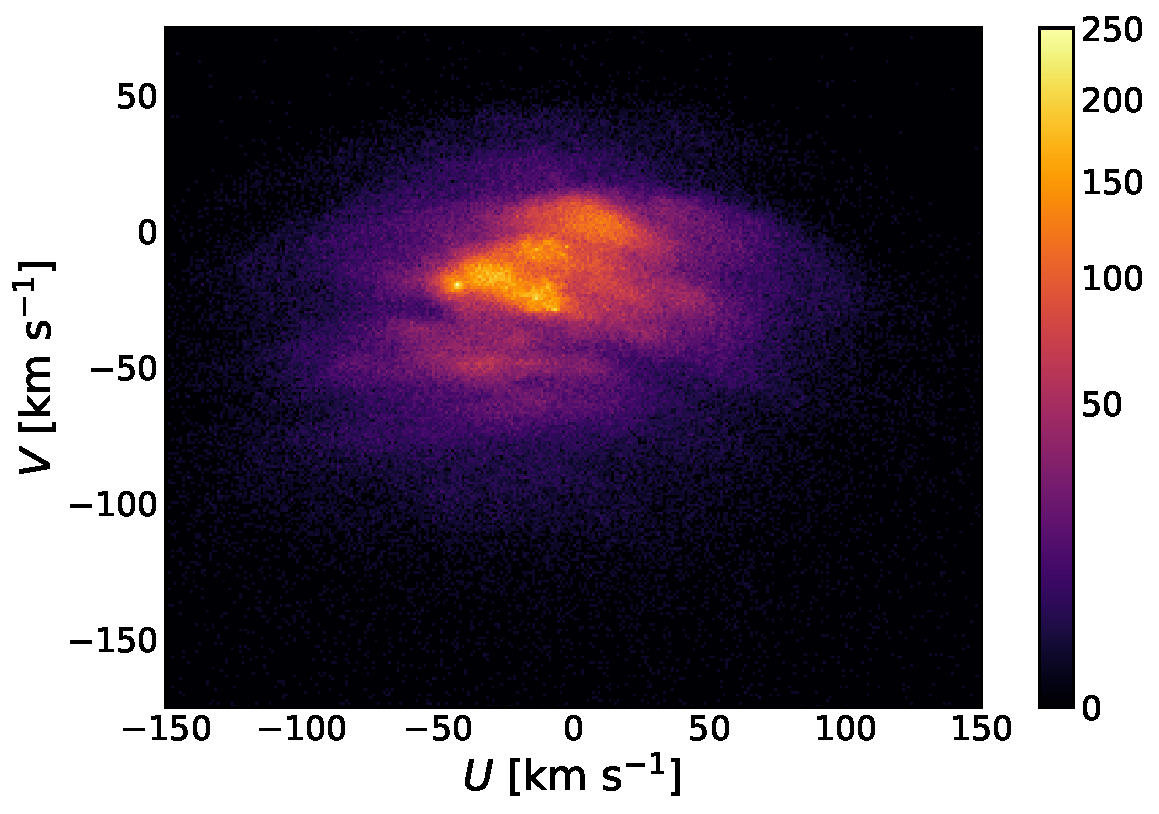
\includegraphics[width=0.8\textwidth]{images/dr3veldist.pdf}
    \caption{The number density distribution of sources from DR3 with radial velocities in the Solar neighbourhood. There is clearly a great deal of structure present already at close proximity to the Sun. The colorscale is shows $\sqrt{N}$ and the axes show Galactic velocities $U$, towards the Galactic centres, and $V$, in the direction of Galactic rotation.} % Fig. 3.2
    \label{fig:veldist}
\end{figure}

Now comes the issue; we do not have 3D velocities for the majority of these sources. How can we hope to determine the velocity distribution? To begin with, we can simply work with the sources that have radial velocities. This has been done of course and for DR2 it was in one of the demonstration papers, \citep{dr2:kinematics}. We use DR3 to recreate the same plot here, using a similar Solar neighbourhood sample we have around 500 000 stars, whereas in DR2 the sample contained {$\sim$}350 000 stars. The velocity distribution can be seen in Fig. \ref{fig:veldist}. This figure shows us that the velocity structure of the Galaxy, even locally, is anything but straight-forward. Structure in velocity space can be caused by a variety of processes \citep[see, e.g.,][]{antoja:10a}. Originally it was thought to come from disrupted stellar clusters. Newer suggestions have been accreted dwarf galaxies and close passings by external galaxies. Last but not least, the resonances of the spiral arms and bar, as discussed in the context of Paper I, can cause substructure in velocity space as well. We can with ease understand how decoding the velocity structure of the Galaxy will provide valuable insight into its evolution and history. It is therefore vital that we have access to as many stars as possible.

So what about the remainder of sources? It turns out that all hope is not lost. Already in \cite{dehnen:98a} the velocity distribution from Hipparcos was determined, despite the lack of radial velocities, by employing a clever approximation of a velocity distribution which is isotropic across the sky and then inferring $f(\bm{v})$ with a penalized maximum likelihood estimate (MPLE) (we will return to this in section \ref{sec:p2-inferring}). Similarly the average velocities and the velocity dispersion were determined in \cite{dehnen:98b}. Other studies that work around the absence of measured radial velocities include \cite{antoja:17} with estimates of disc velocity asymmetries, \cite{koppelman:21} who determined the Milky Way's escape velocity, and \cite{mcmillan:22} who looked to the outer parts of the disc near the anti-centre and showed that the velocities exhibit properties that match well with being perturbed by a dwarf galaxy. At least for now, it is absolutely necessary to use proper motion-limited samples if we wish to have access to catalogues that span a greater part of our Galaxy, and if we wish to have access to all kinds of stars. 

The astrometric renaissance is now and it is an exciting time for all fields of astronomy that can make use of the impressive data that is not only currently released, but is sure to arrive in the foreseeable future.
